{\let\clearpage\relax\let\cleardoublepage\relax
%\chapter{Modelli di formazione globali e semplificazioni introdotte}
\chapter{Popolazioni planetarie sintetiche e confronto con osservazioni}
}
(Vedi \cite{mordasini2009extrasolar}, \cite{mordasini2018planetary})

\begin{workout}[Mordasini18 MAIN RESULTS]
	\begin{itemize}
		\item Cosa ho messo nel modello e2e? (Montecarlo variables) Disk metallicity $[M/H]$ (Santos 05) and $f_{dg}$ (Lodders 03). Initial disk mass: stability (SHu 90), observation (andrws 10, manara 16) MMSN; Disk lifetime (Haisch 01, mamajek 09); starting embryos position
		planetesimal size is 300m, planetesimal distro $\propto r\expy{-1.5}$ and outer exponential radius half that of gas to account inward drift (kornet 01; birnstiel andrews 14) and more concentrated distro resulting from planetesimal formation (drazkowska 16) - ''The TW Hya Disk at \SI{870}{\micro\meter}:  Comparison of CO and Dust Radial Structures'' 2011; planetesimal size 300m: what's influenced?
		Struttura disco accrescimento: calibrazione tempo di vita, evoluzione viscosa ed evaporazione - $\alpha=0.002$.
		Evoluzione embrioni: accrescimento, evoluzione orbitale (N-body+migration timescale+e,i damping)
		
		\item Distribuzione massa pianeti: distribuzione bimodale con discrimine a $30\mearth{}$.
		\begin{figure}[!ht]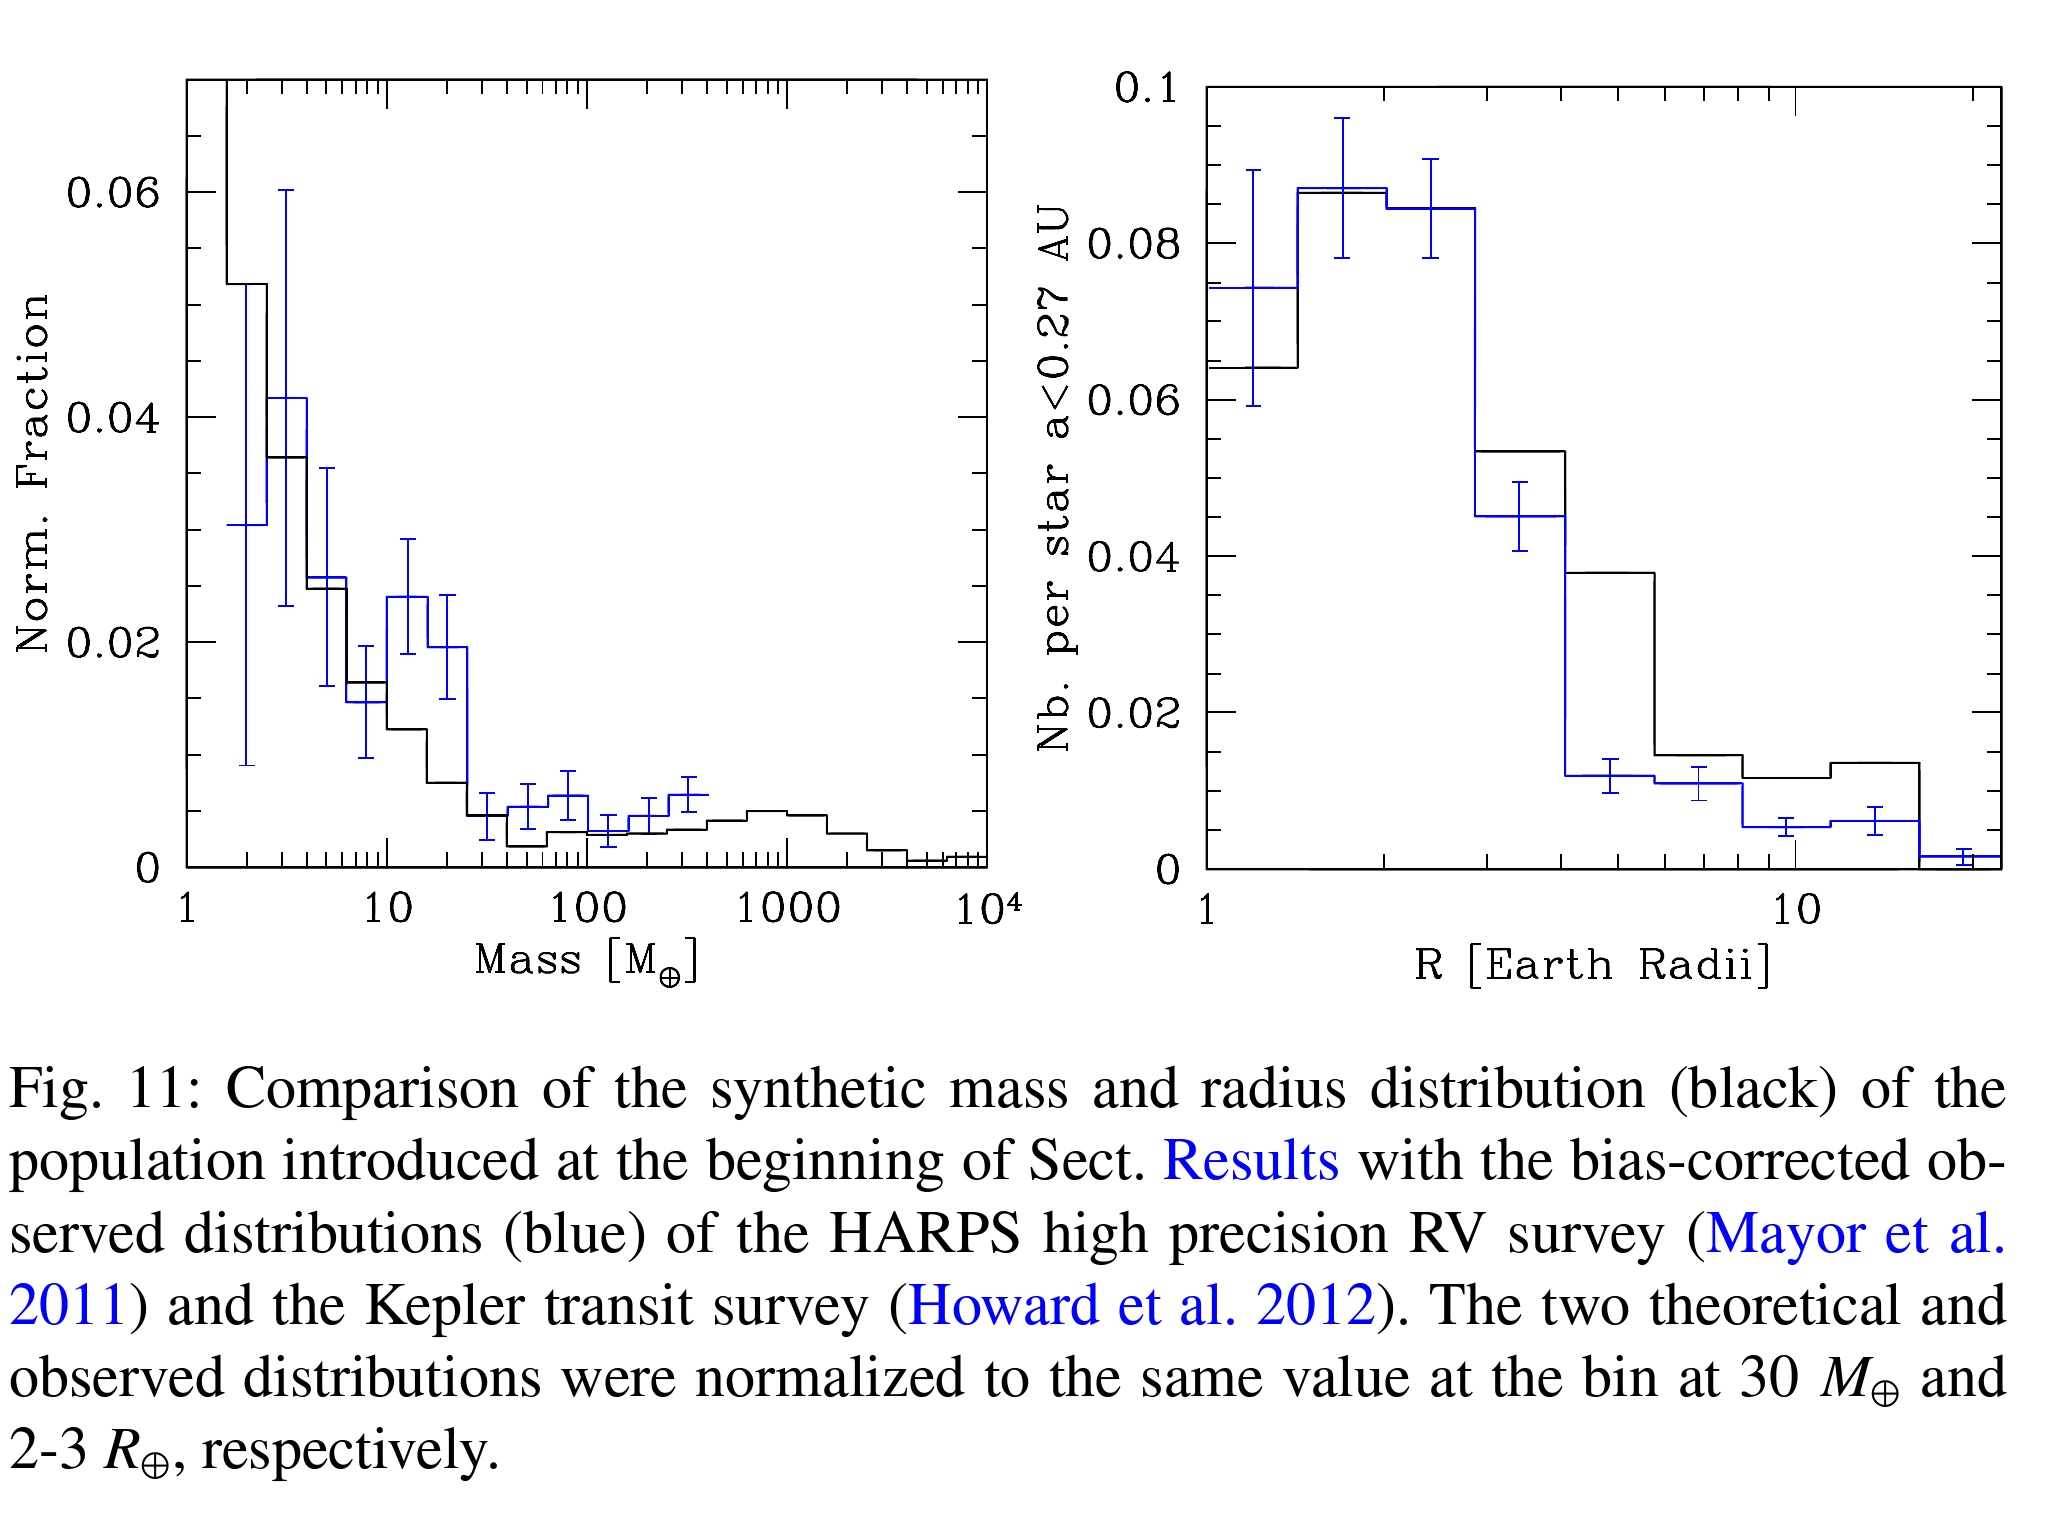
\includegraphics[trim={0cm 17cm 0 0},clip, keepaspectratio,width=0.9\textwidth]{MR-freq-obssynth}\caption{Distribuzioni di massa e raggio per popolazione planetaria sintetica (linea nera) e distribuzioni osservate tramite RV e transiti (linea blu) corrette per i bias. Da \cite{mordasini2018planetary}.}\label{fig:MR-freq-obssynth}\end{figure}
		Massa critica per accrescimento di gas: tempo scala accrescimento planetesimi vs tempo scala disco.
		Tempi scala migrazione
		\item distribuzione in semiassi che dipende da posizione iniziale embrione: necessity to include earlier planetary formation; montecarlo variable: initial starting position embryos- kokubo ida 00: uniform distro in log(a) (vedi anche ida lin 10) (dov'era scritto del comportamento caotico??+); hasegawa pudritz 11, cridland 16: embryos rapidly moves into traps.
		Preferred formation regions of planetesimal (Drazkowska16; brauer 08), particle pile-up outside orbits of already existing planets (Pinilla15), strong migration traps (Horn 12, Hasegawa Pudritz 12).
		Disc/planetesimals parameters: planetesimal has steeper profile $\propto r\expy{-3/2}$, outer exponential radius half that of gas: inward drift of dust (kornet 01, birnstiel Andrews 14), concentrated distro resulting from planetesimal formation (Drazkowska 16);
		\item Distribuzione raggi: diagramma massa-raggio, composizione, evaporazione.
		\item (Mordasini pg 27) LArge majority are low mass planets ($0.1-10\mearth{}$), 
		\item frequency of giant, close-in and habitable planets. The high frequency of close-in planets can be reproduced assuming steep distribution of planetesimal and centrally concentrated (chiang laughlin 13, drazkowska 16)
		\item correlation with disk properties (mordasini 12a): metallicity effects (mortier13)
		\item Sub-saturn mass desert (ida lin 04) not seen in kepler data (Thompson 18): accretion of planetesimal slow down gas accretion
		\item migrazione, cattura risonante: ''On the migration of two planets in a disc and the formation of mean motion resonances'' Migaszewski 15; ''Perturbation of compact planetary systems by distant giant planets'' Hansen 17
	\end{itemize}
\end{workout}

\begin{errata}[planetary system diversity]
	Il variare delle caratteristiche dei sistemi planetari osservati \'e determinato dal variare delle condizioni iniziali: distribuzione di massa dei dischi protoplanetarii e di metallicit\'a, tempo di vita, condizioni del cluster di cui fa parte il disco.
\end{errata}

Le popolazioni planetarie sintetiche sono costruite partendo dalla fase finale di accrescimento di massa sulla stella centrale. Data la molteplicit\'a delle scale dimensionali dei fenomeni che portano alla formazione planetaria \'e necessario introdurre una descrizione semplificata di questi; quindi generare una popolazione planetaria a partire da un gran numero di combinazioni di condizioni iniziali determinate casualmente con distribuzione in accordo alle osservazioni. In questo modo \'e possibile determinare in maniera statistica l'accuratezza delle ipotesi su cui si basano i modelli di formazione planetaria tramite confronto con la distribuzione delle propriet\'a dei pianeti osservati, tenuto conto dei bias osservativi e della distribuzione delle condizioni iniziali.

\section{Modello di Berna}


\begin{figure}[!ht]
	\begin{subfigure}{0.5\textwidth}
		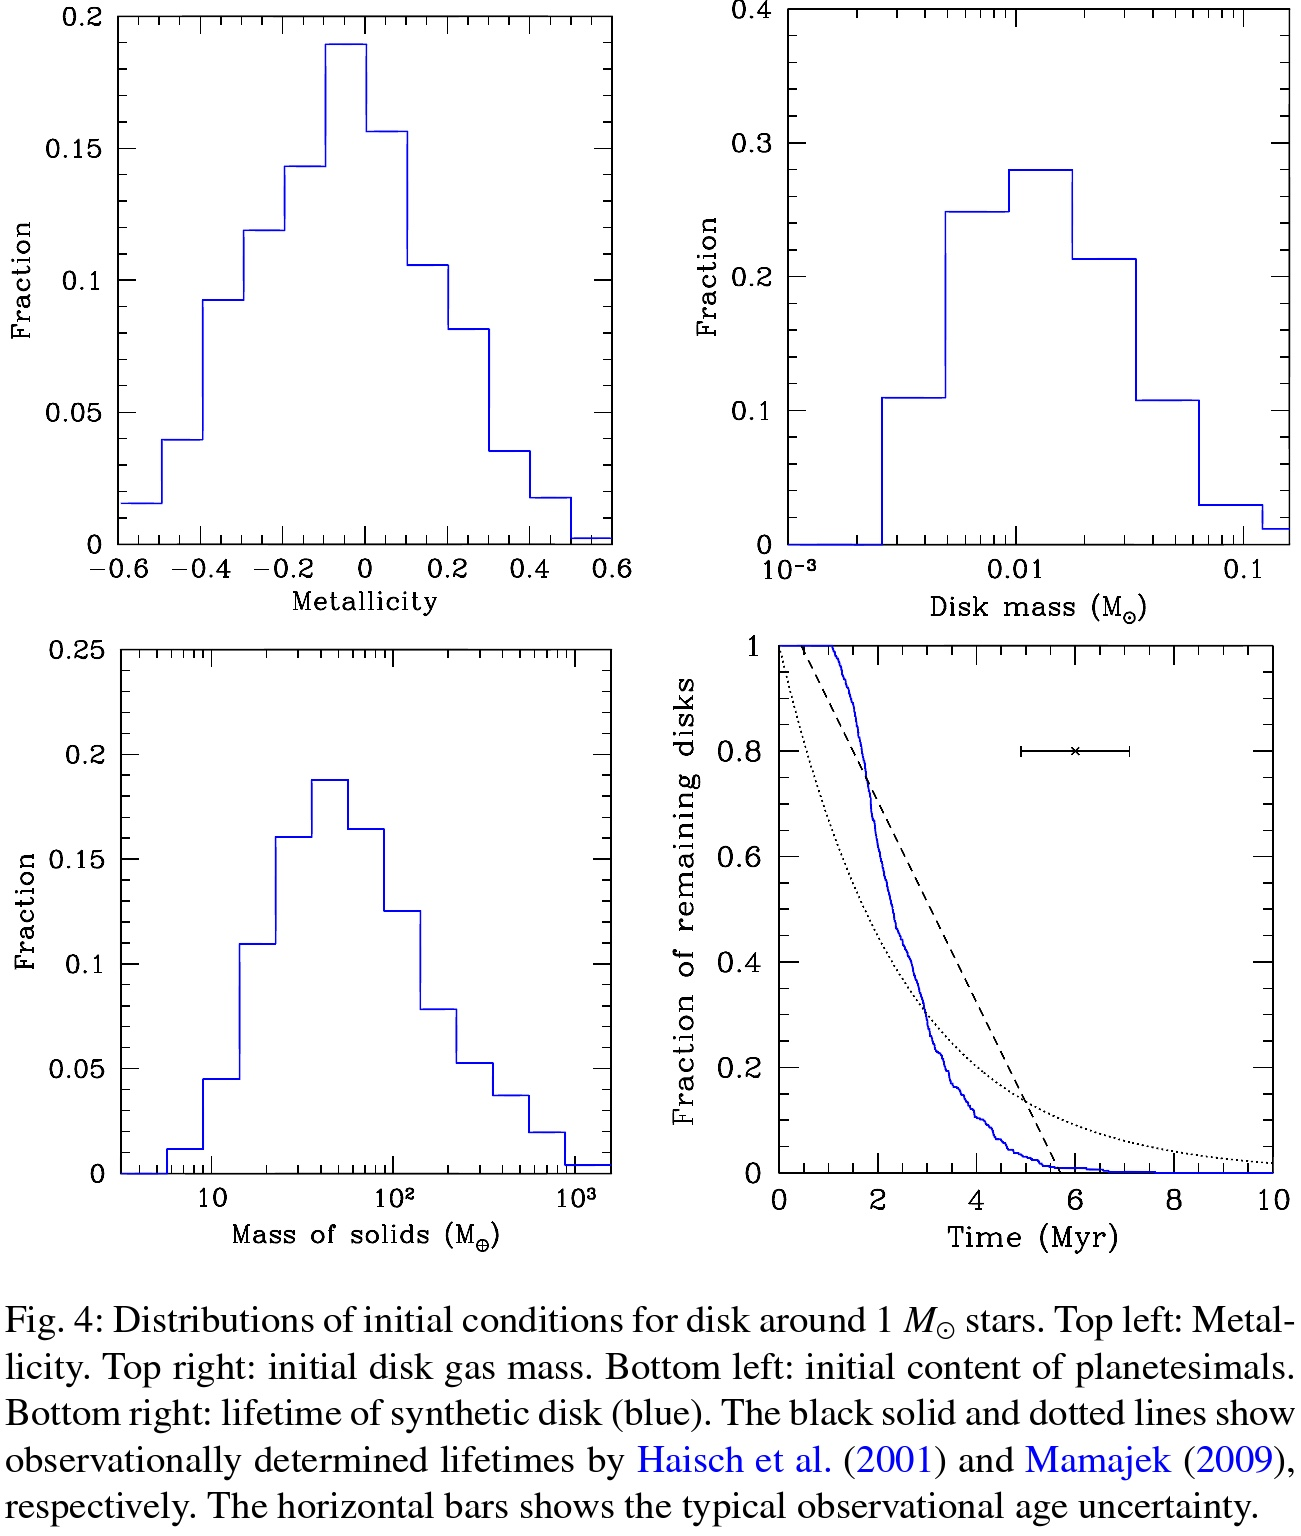
\includegraphics[trim={0cm 10cm 0 0},clip, keepaspectratio,width=0.99\textwidth]{initdistro}
	\caption{Distribuzione caretteristiche dischi di accrescimento. Da \cite{mordasini2018planetary}.}\label{fig:initdistro}
	\end{subfigure}
\begin{subfigure}{0.5\textwidth}
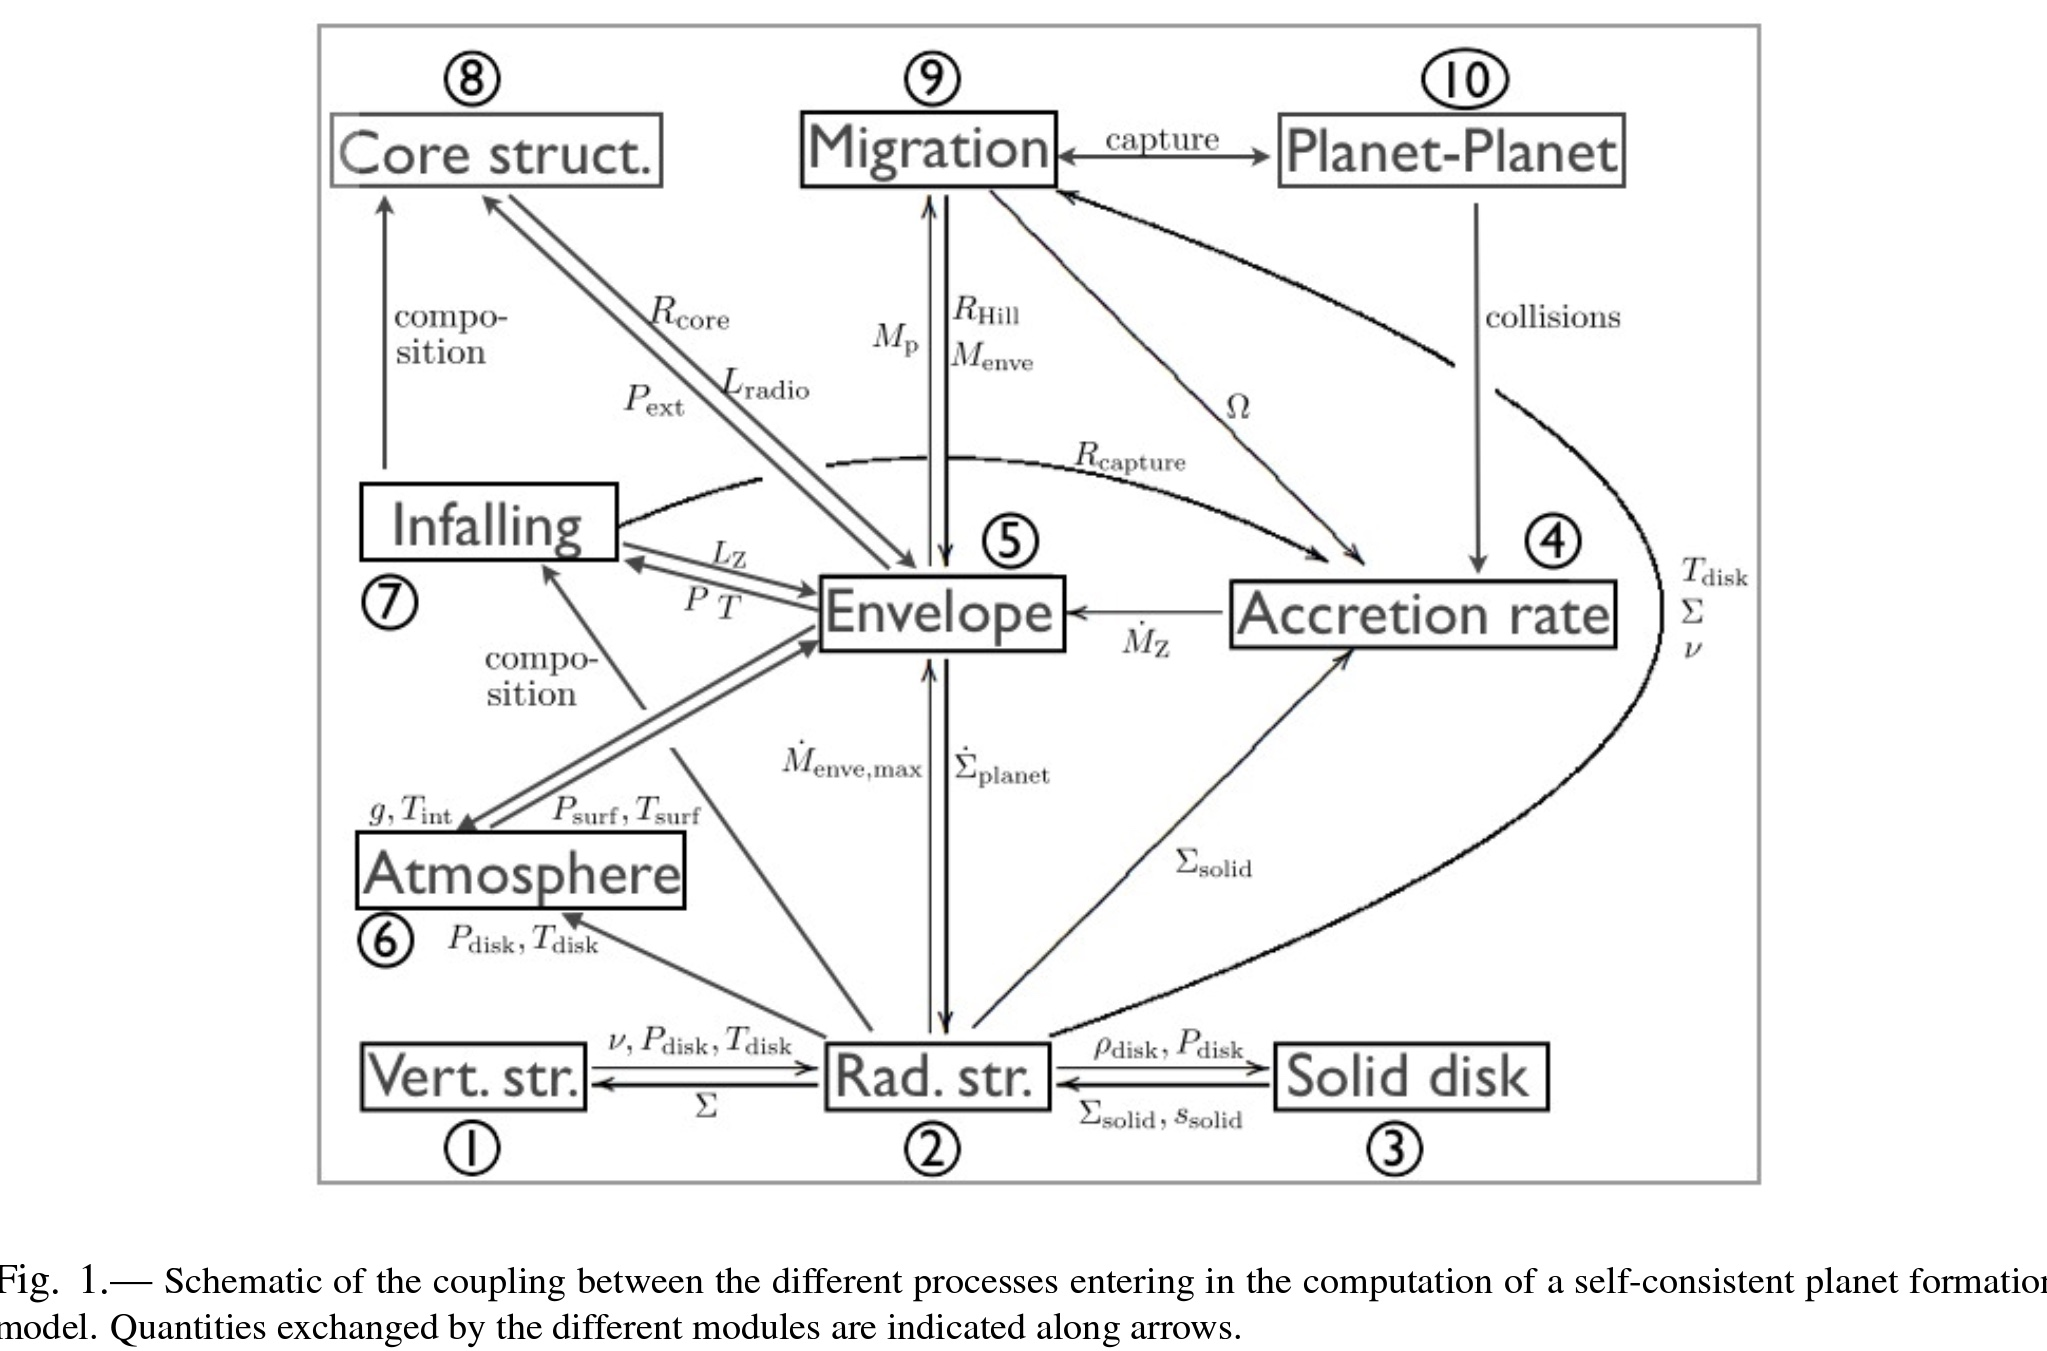
\includegraphics[trim={9cm 5.5cm 10cm 0.5cm},clip, keepaspectratio, width=0.99\textwidth]{GFM}
\caption{Schema dei processi che \'e necessario includere in un modello di formazione planetario coerente.
	Da \cite{benz2014planet}.}\label{fig:GFM}
\end{subfigure}
\end{figure}

%\begin{wrapfigure}[22]{l}{0.7\textwidth}

La struttura del disco protoplanetario determina la rapidit\'a di accrescimento degli embrioni planetari  principalmente tramite la densit\'a di planetesimi: posizione dell'iceline ($H_2O$) fissa \'e coerente con assunzione di trasformazione totalit\'a componente solida in planetesimi.
\'E possibile tenere traccia della frazione di rocce o ghiacci accresciuti: la figura \ref{fig:MR5Gyrppsobs} mostra la posizione nel diagramma massa-raggio di una popolazione sintetica con quella di pianeti reali. La fase di contrazione post-formazione \'e determinata considerando l'evoluzione de

%LBRT
\begin{figure}[!ht]
		\centering
		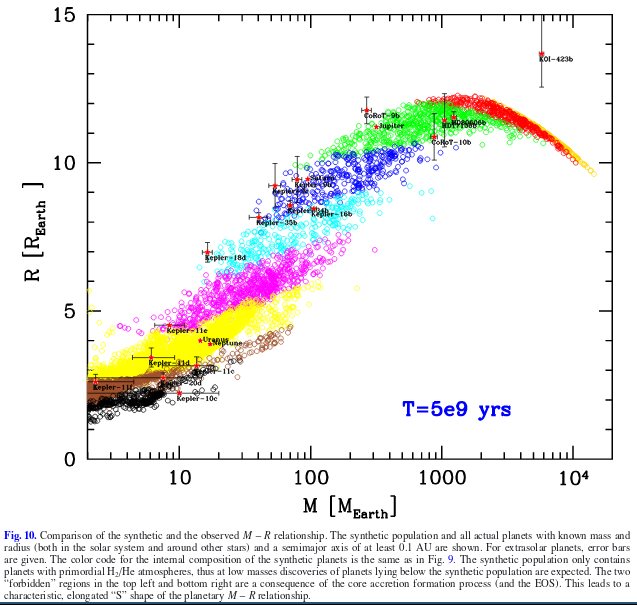
\includegraphics[trim={0.8cm 2.8cm 0.5cm 0.4cm},clip, width=0.99\textwidth,keepaspectratio]{MR5Gyrppsobs}
		\caption{Popolazione planetaria sintetica nel diagramma massa-raggio a $t=\SI{5}{\giga\year}$. Colore indica frazione di metalli: Arancio $Z<1\%$, Rosso $1\%<Z<5\%$, Verde $5\%<Z<20\%$, Blu $20\%<Z<40\%$, Celeste $40\%<Z<60\%$, Magenta $60\%<Z<80\%$, Giallo $80\%<Z<95\%$, Marrone $95\%<Z<99\%$, Nero $Z>99\%$. Da \cite{mordasini2012characterizationmassradius}. }\label{fig:MR5Gyrppsobs}
\end{figure}

\begin{workout}[Radius of planet diminish as core mass increases]
Characterization of exoplanets from their formation I:  radii pg 15
\end{workout}

Lo scambio di momento angolare dovuto all'interazione gravitazionale tra disco e pianeta provoca la migrazione planetaria 

Se l'embrione planetario accresce abbastanza massa si forma un inviluppo gassoso che inzialmente si raccorda alle condizioni del disco e alla saturazione della capacit\'a del disco di fornire gas si stacca dal disco: la struttura del pianeta \'e quindi determinata da massa, raggio e luminosit\'a del core, massa gassosa legata al pianeta, energia rilasciata da accrescimento planetesimi e gas.

%La capacit\'a del pianeta di accrescere planetesimi aumenta con l'aumentare della massa e del raggio del pianeta.

\begin{errata}[atmosfera e luminosit\'a pianeta: discorsivo]
 Le condizioni in fondo all'atmosfera planetaria forniscono le condizioni di temperatura e pressione all'estremo dell'inviluppo gassoso. La struttura del disco determina anche il rate massimo di accrescimento del gas. Il rate d'accrescimento di solidi \'e determinato dalla sezione d'urto efficace, determinata dalla struttura dell'inviluppo gassoso, dalla densit\'a di solidi nel disco e dalla velocit\'a orbitale. La luminosit\'a del pianeta \'e determinata dal rate di accrescimento dei solidi e dal rate di contrazione del pianeta. Infine la migrazione \'e determinata dalla caretteristiche del disco e dalla massa del pianeta.
\end{errata}

\begin{workout}[Distribuzione raggi pianeti giganti e opacit\'a]
Burrows 07
\end{workout}

\begin{workout}[bloating effect]
baruteau 16
\end{workout}

\begin{workout}[Ref PPS]
Towarddeterminist model of planetary formation iV: effectsof type I migration
									: accumulation neare iceline
									: dynamical intaraction and coagulation of multiple rocky embrios (isolation mass, semi-analytic vs n-body)
									: eccentricity distribution of gas giant
Theoretical models of planetary system formation: mass vs. semi-major axis	(alibert carron 13)			Lecture 15 -planetary ...
Modelling planetary system formation with N-body simulation (11)
Global model of planet formation and evolution
Planetary population synthesis
planet population synthesis					
\end{workout}

%\section{Popolazioni planetarie sintetiche}
%Considero i risulati di alcuni modelli di formazione planetari (\cite{mordasini2018planetary}).
\begin{errata}[Soluzione del modello di formazione globale]
La soluzione del modello di formazione planetario variando le condizioni iniziali in maniera opportuna e determinando un gran numero di combinazioni tramite metodi di montecarlo produce un ensemble di sistemi da cui, tramite confronto statistico con la popolazione osservata, si valuta l'accuratezza delle .
\end{errata}

%\subsection{Progresso nei modelli di formazione globale}

\begin{workout}[Risultati dello sforzo di riprodurre la forma del diagramma a-M]
Alcuni risultati prodotti dal tentavo di migliorare l'accordo tra popolazioni sintetiche  e popolazione pianeti reali:
\begin{itemize}
\item Il modello di migrazione GT80 e tanaka02 producono migrazipone troppo veloce (mordasini09: assenza pianeti minori di 10masse solari entro 0.1AU). L'analisi del momento torcente di corotazione in dischi non isotermi dimostra che questo fenomeno pu\'o essere la soluzione alla migrazione troppo rapida, inoltre si pu\'o avere migrazione verso l'esterno con formazione di zone di convergenza.
\item rate di accrescimento di gas runaway (ida lin 04: deserto di pianeti tra 10-100 masse terrestri): il calore generato dall'accrescimento di pianetesimi ritarda l'accrescimento di gas e nei modelli recenti i a molti embrioni si ha competizione per il gas
%\item Migrazione II: flussi di gas
\item molteplicit\'a: effetti sui pianeti di piaccola massa sono scattering (eccitazione eccentricit\'a o espulsione), cattura in risonanza e collisioni
\item Relazione con massa stellare: Stelle di minor massa sono circondate da dischi di minore massa: quindi minor frequenza di giaganti.%Relazione tra $\eta_J-M_*$
\end{itemize}
\end{workout}

%\subsection{Popolazione M18}

\begin{figure}[!ht]
\centering
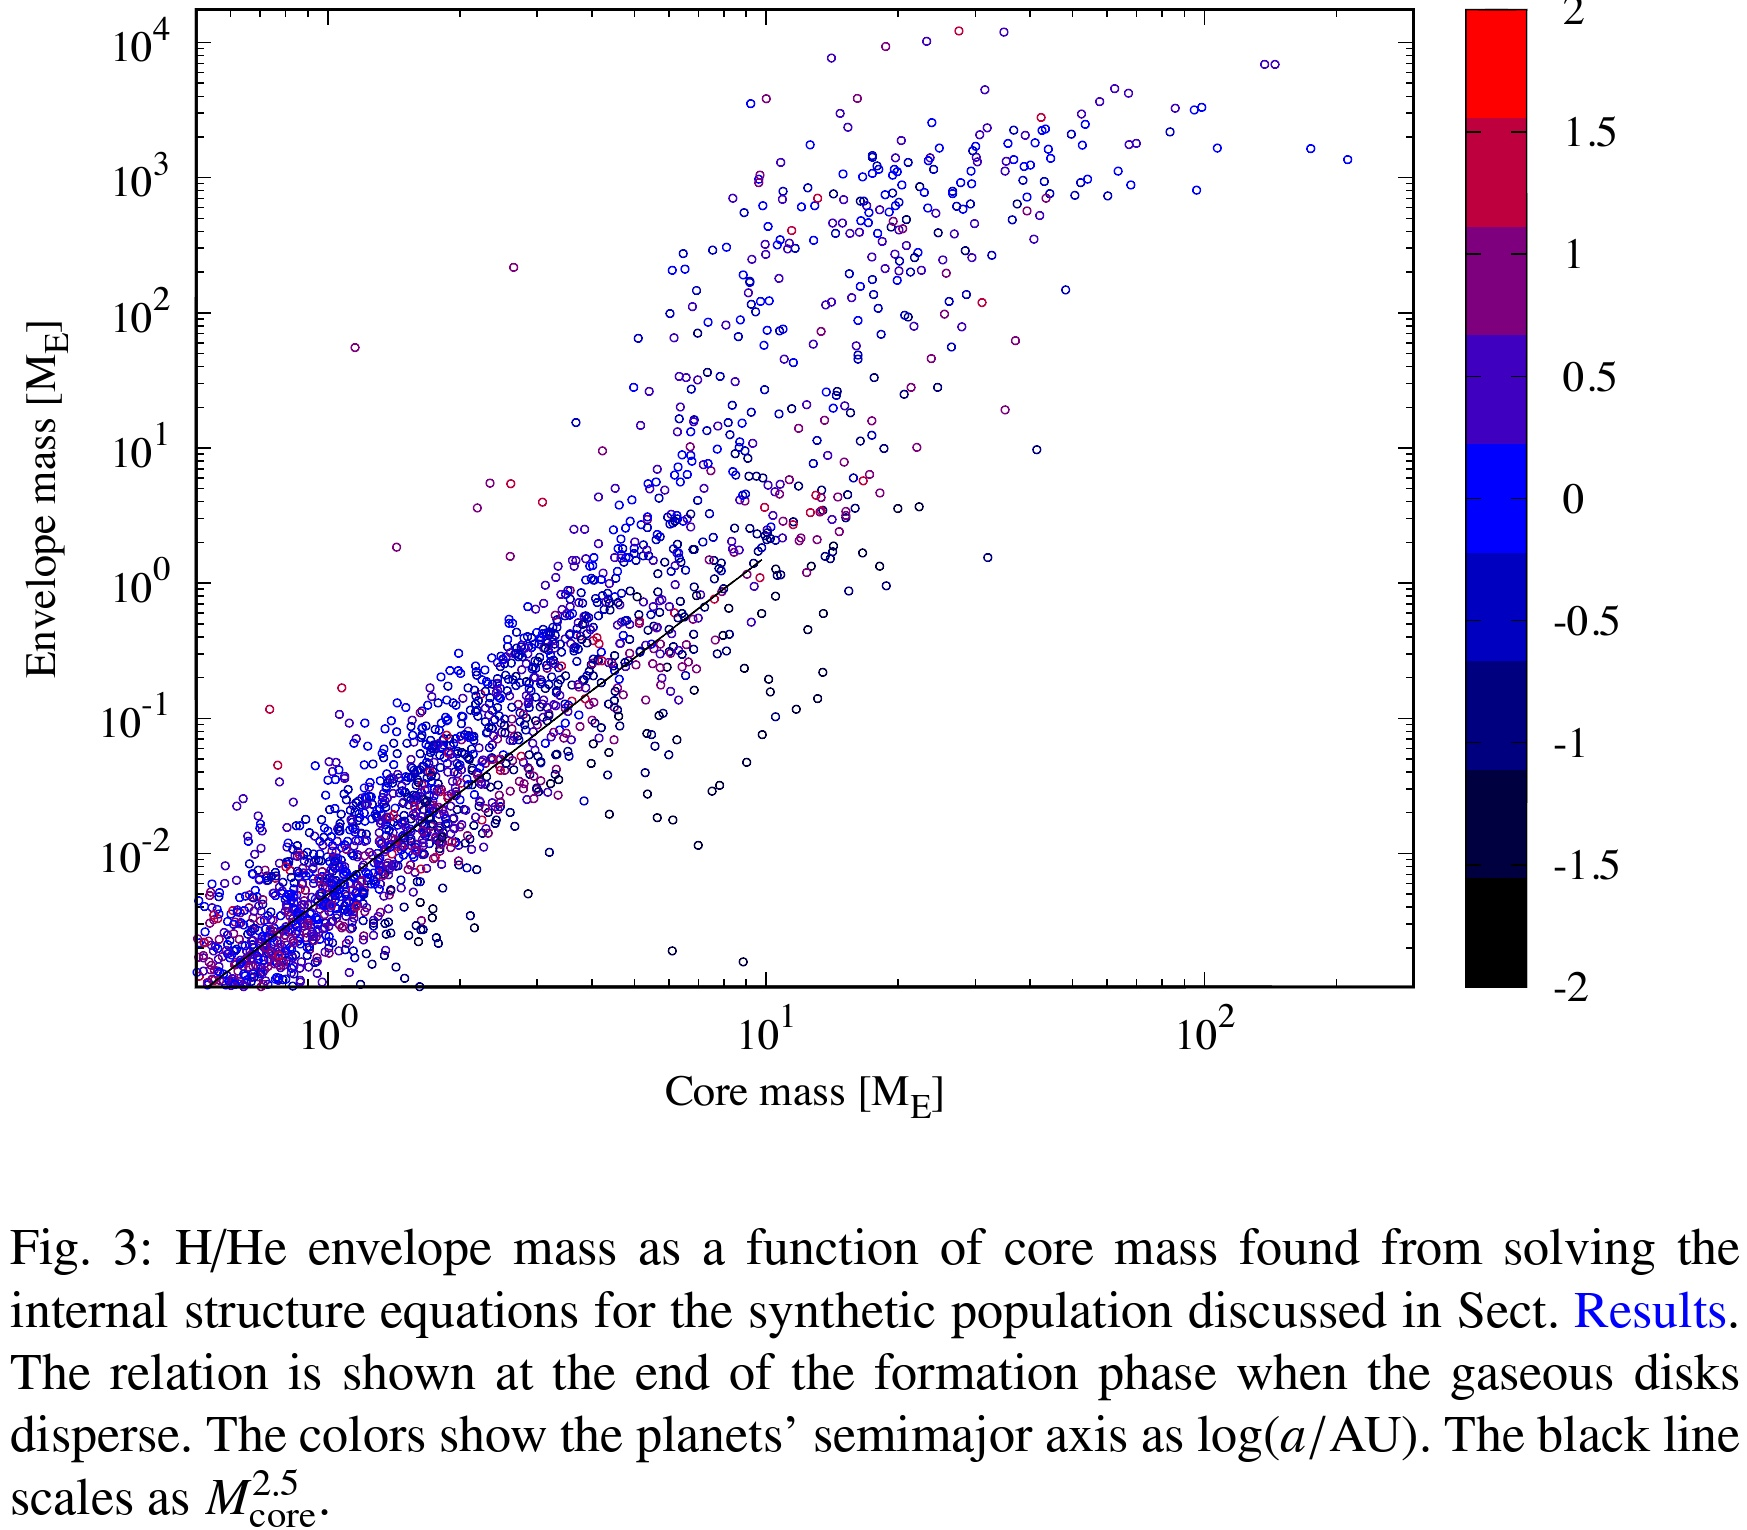
\includegraphics[trim={0cm 12cm 0 0},clip, width=0.9\textwidth,keepaspectratio]{envelopecoresynth}
\caption{Massa inviluppo gassoso vs massa core. Il colore indica la distanza in $\log{\frac{a}{\si{\astronomicalunit}}}$. La linea continua mostra andamento $M_c\expy{-q_{KH}-1}=M_c\expy{2.5}$ precedente alla fase runaway di accrescimento gassoso. Da \cite{mordasini2018planetary}. }\label{fig:envelopecoresynth}
\end{figure}

La figura (\subref{fig:ma-synth}) mostra la distribuzione della popolazione sintetica nel diagramma massa-distanza: la posizione finale di un pianeta \'e terminata principalmente dai tempi caratteristici di accrescimento e migrazione; considerando inoltre l'interazione gravitazionale tra i pianeti si hanno effetti delle risonanze e eccitazione di eccentricit\'a.

\begin{figure}[!ht]
\begin{subfigure}[b]{0.5\textwidth}
\centering
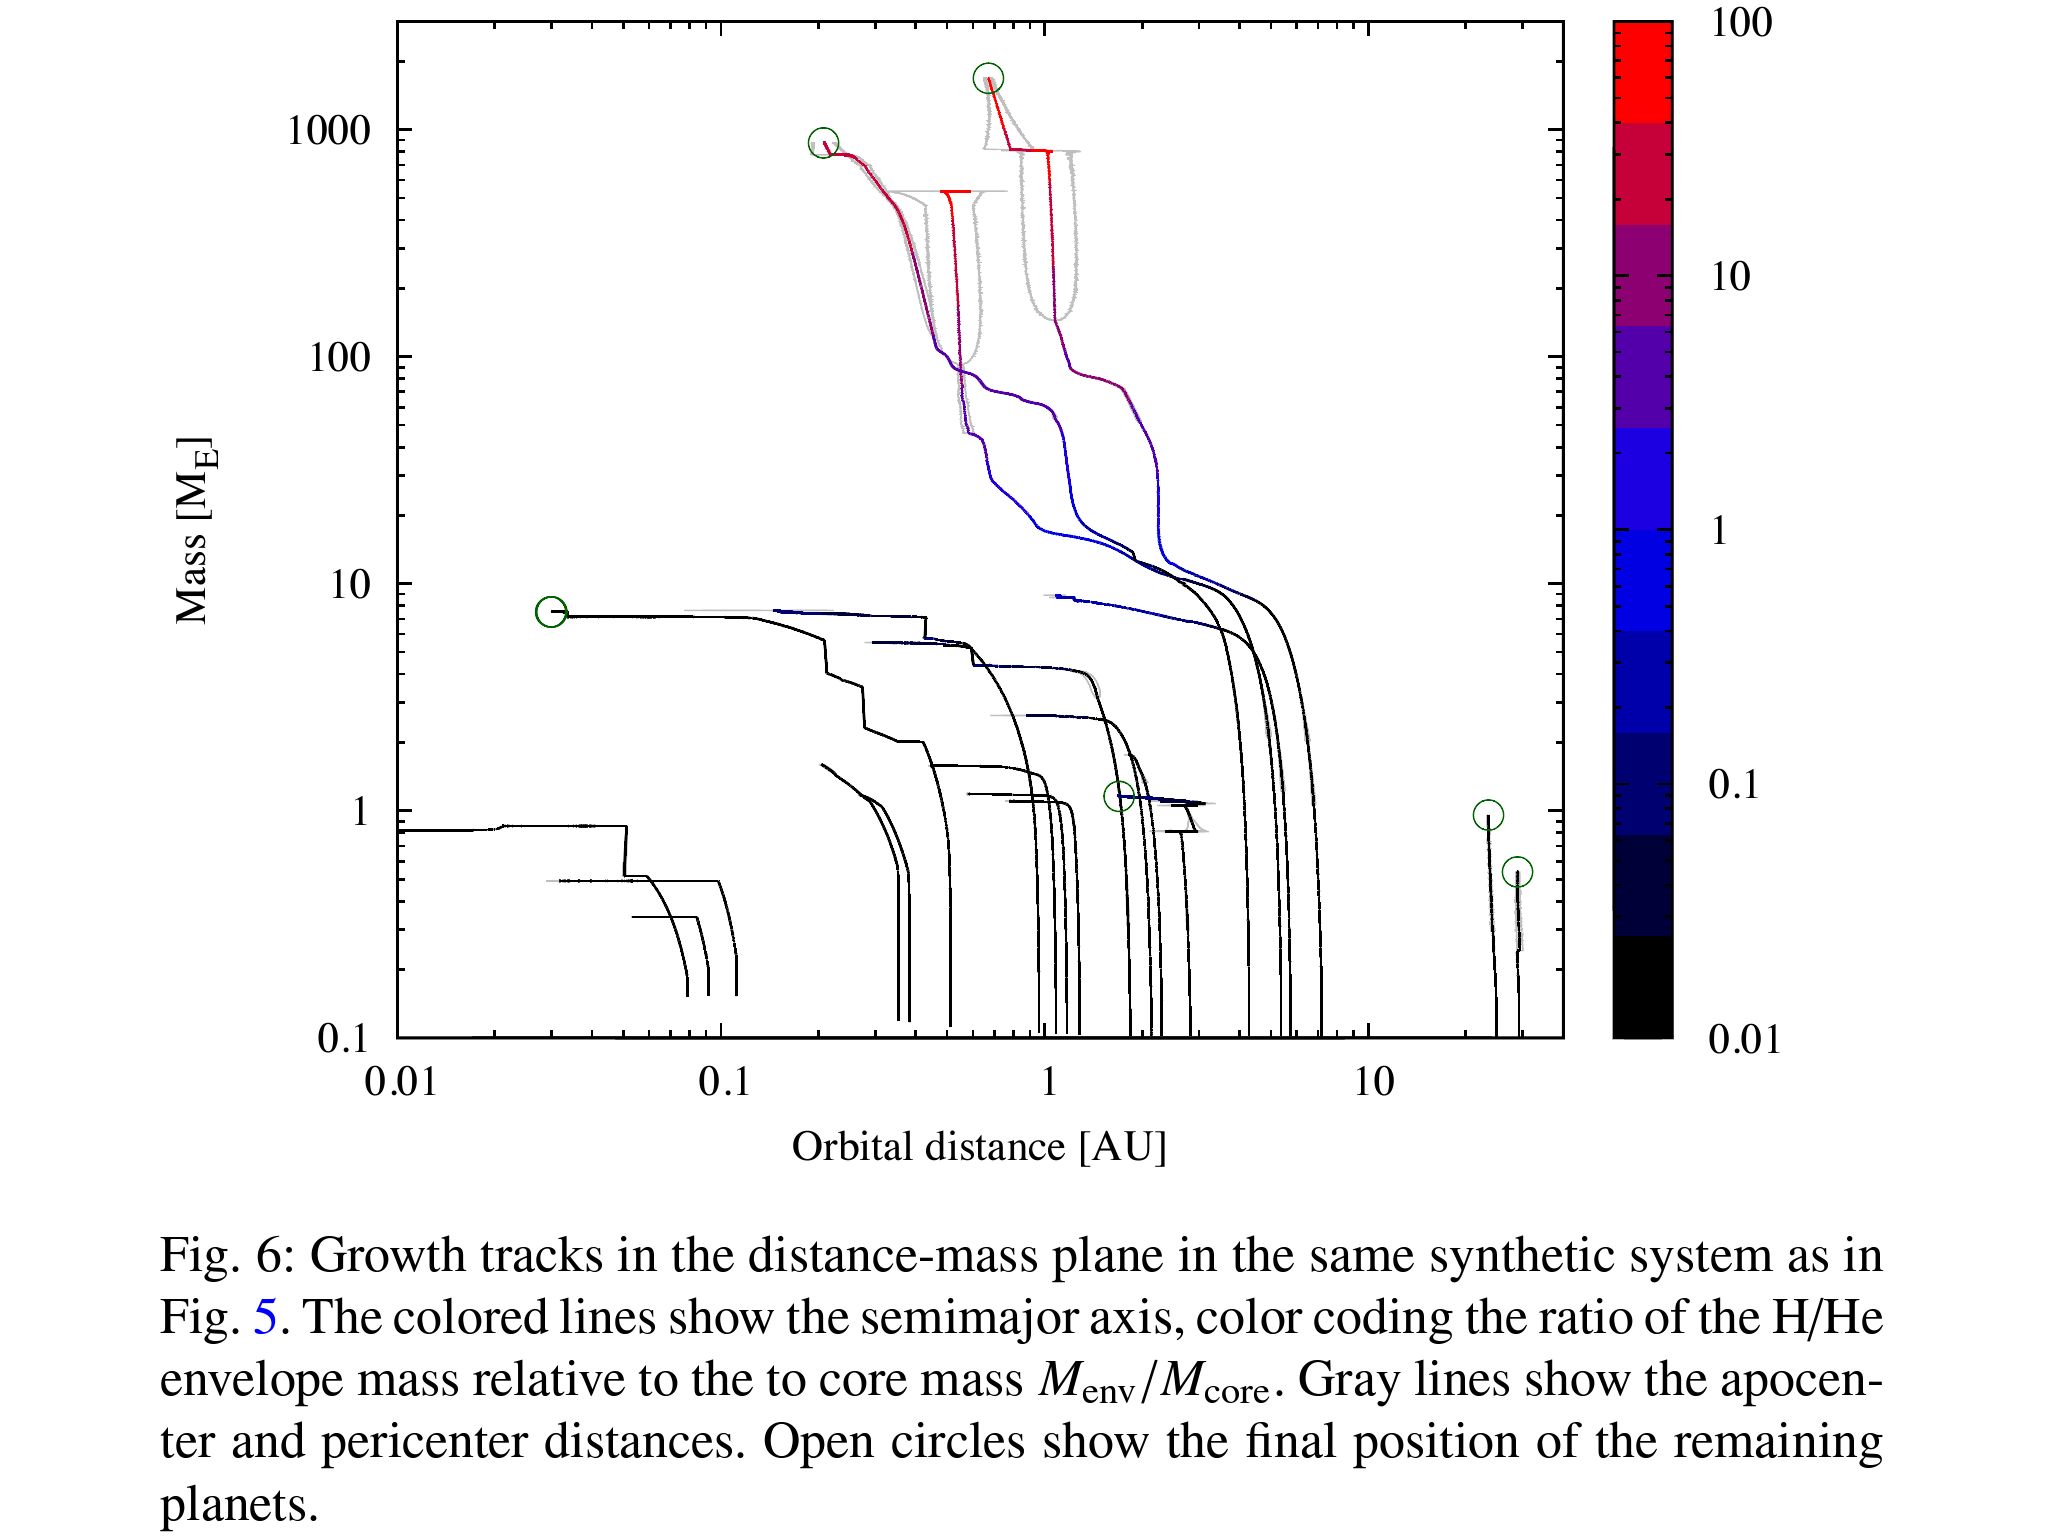
\includegraphics[trim={6cm 13cm 7cm 0.5cm},clip, width=\textwidth,keepaspectratio]{track1}
\caption{Formazione di un sistema planetario nel diagramma $a-M$: alla scomparsa del disco protoplanetario si hanno 2 pianeti giganti, un nettuniano caldo e 3 pianeti terrestri. La scala di colore indica la composizione $\frac{M_e}{M_c}$. Da \cite{mordasini2018planetary}.}\label{fig:track1}
\end{subfigure}
~
\begin{subfigure}[b]{0.5\textwidth}
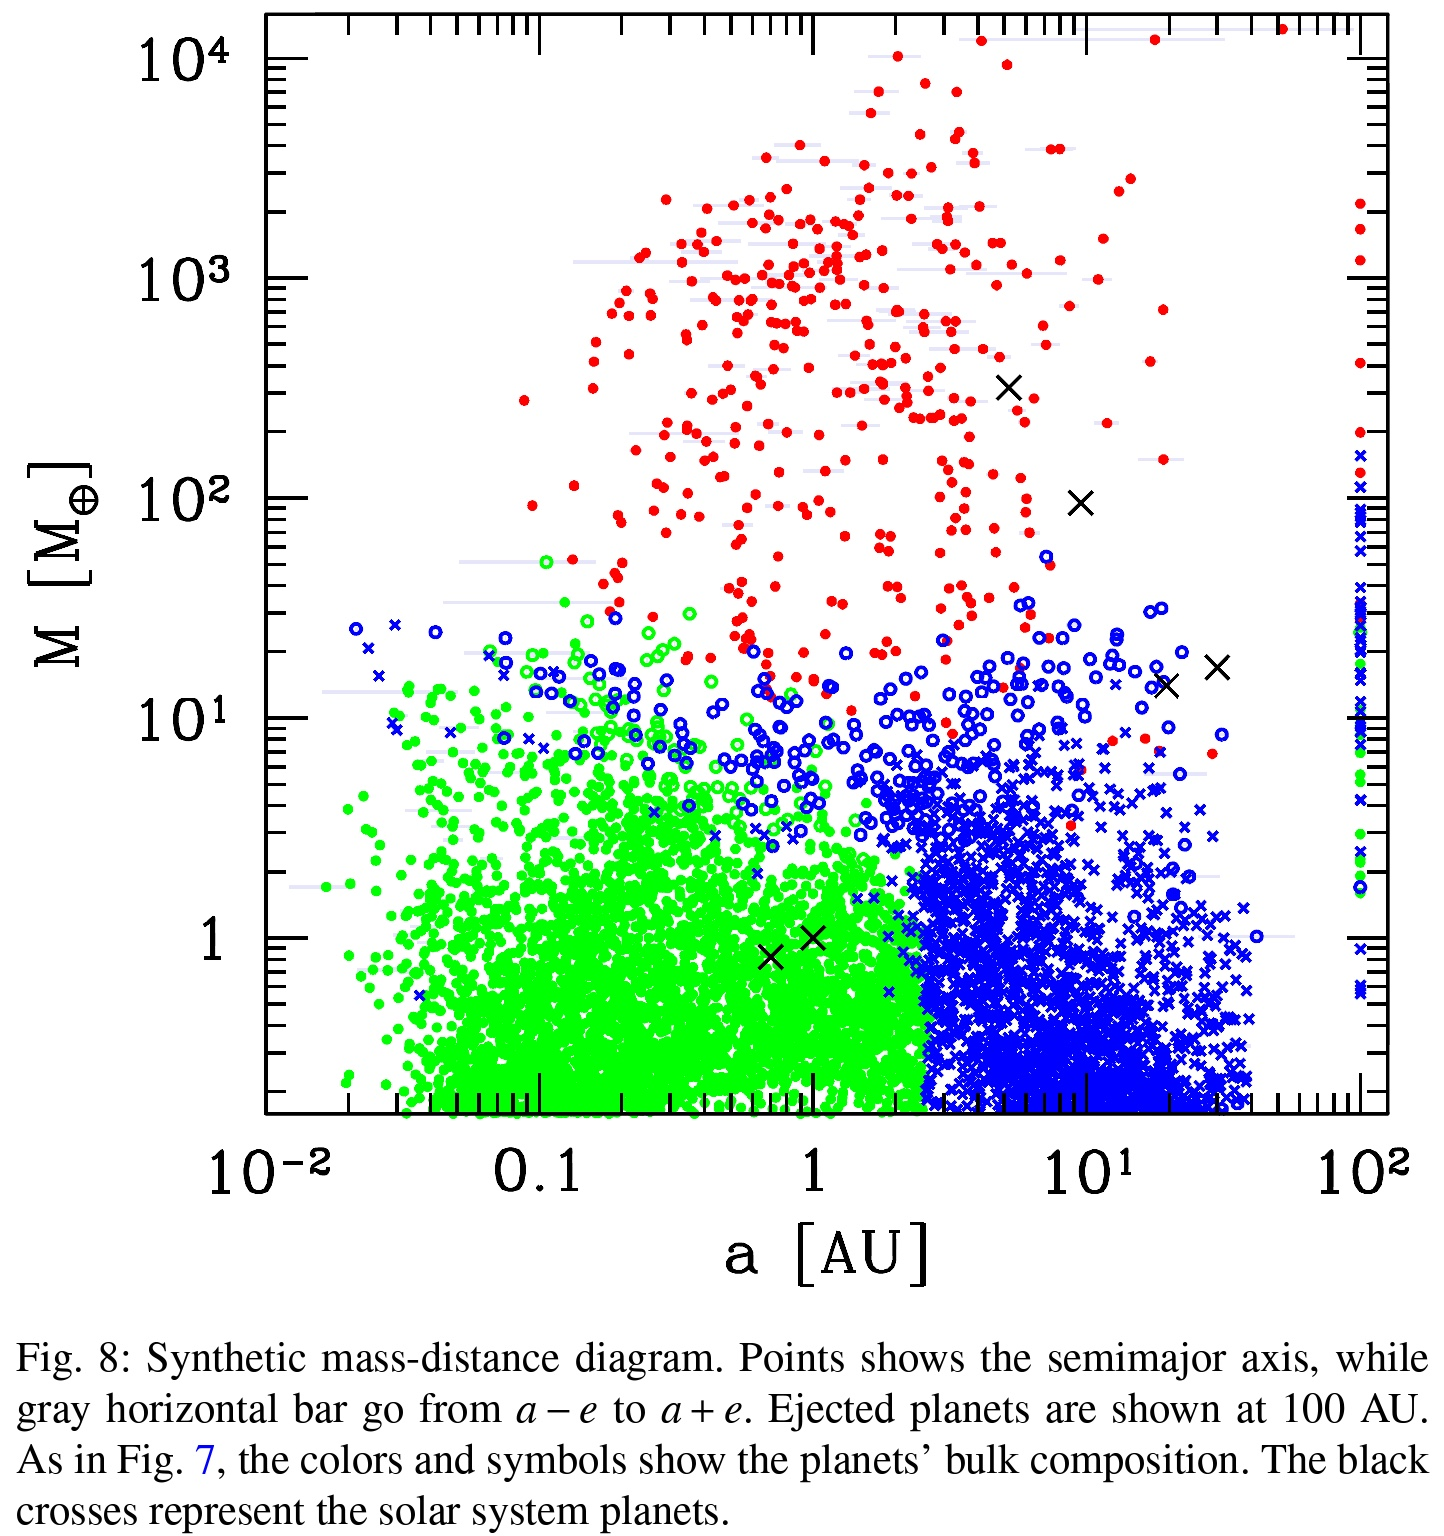
\includegraphics[trim={1cm 9cm 1cm 0},clip, width=0.99\textwidth,keepaspectratio]{ma-synth}
\caption{Simulazione popolazione planetaria di 504 sistemi Punti rossi: pianeti giganti con $M_e/M_c>1$; simboli blu/verdi: pianeti che hanno accresciuto core con ghiacci/rocce; punti aperti: $0.1\leq M_{env}/M_{core}\leq1$; croci blu e punti pieni verdi: pianeti con $M_{env}/M_{core}\leq0.1$. Da \cite{mordasini2018planetary}.}\label{fig:ma-synth}
\end{subfigure}
\end{figure}

Alcune caratteristiche dell'ensemble sintetico: %(\cite{mordasini2018planetary}):
\begin{itemize}
\item Numerosi sistemi costituiti da pianeti di piccola massa (\numrange{0.1}{10}$\mearth{}$)
\item Sistemi con pianeti di piccola massa e giganti. Sistemi che mimano il sistema solare con andamento di massa piccolo-massiccio-piccolo (sweet spot per formazione di pianeti giganti \'e all'esterno dell'ice-line).
\item L'architettura dei pianeti giganti varia notevolmente ma quello pi\'u vicino alle stella \'e distanza di circa \SI{1}{\astronomicalunit}, o meno, dalla stella.
\item Piccola percentuale di sistemi con un pianeta gigante superstite di scattering tra pianeti giganti vicini. Sistemi rari formati in dischi massicci con alta metallicit\'a.
%\item Popolazione di pianeti tra $\numrange{30}{100}\mearth{}$: i fattori che influenzano la popolazione di pianeti di massa intermedia sono la massa presente nel disco quando il protopianeta raggiunge la massa critica per accrescimento di gas, il tempo-scala di rilassamento radiativo e competizione per accrescimento di gas tra protopianeti giganti.
\end{itemize}
%saturazione momento di corotazione

	\begin{figure}[!ht]
	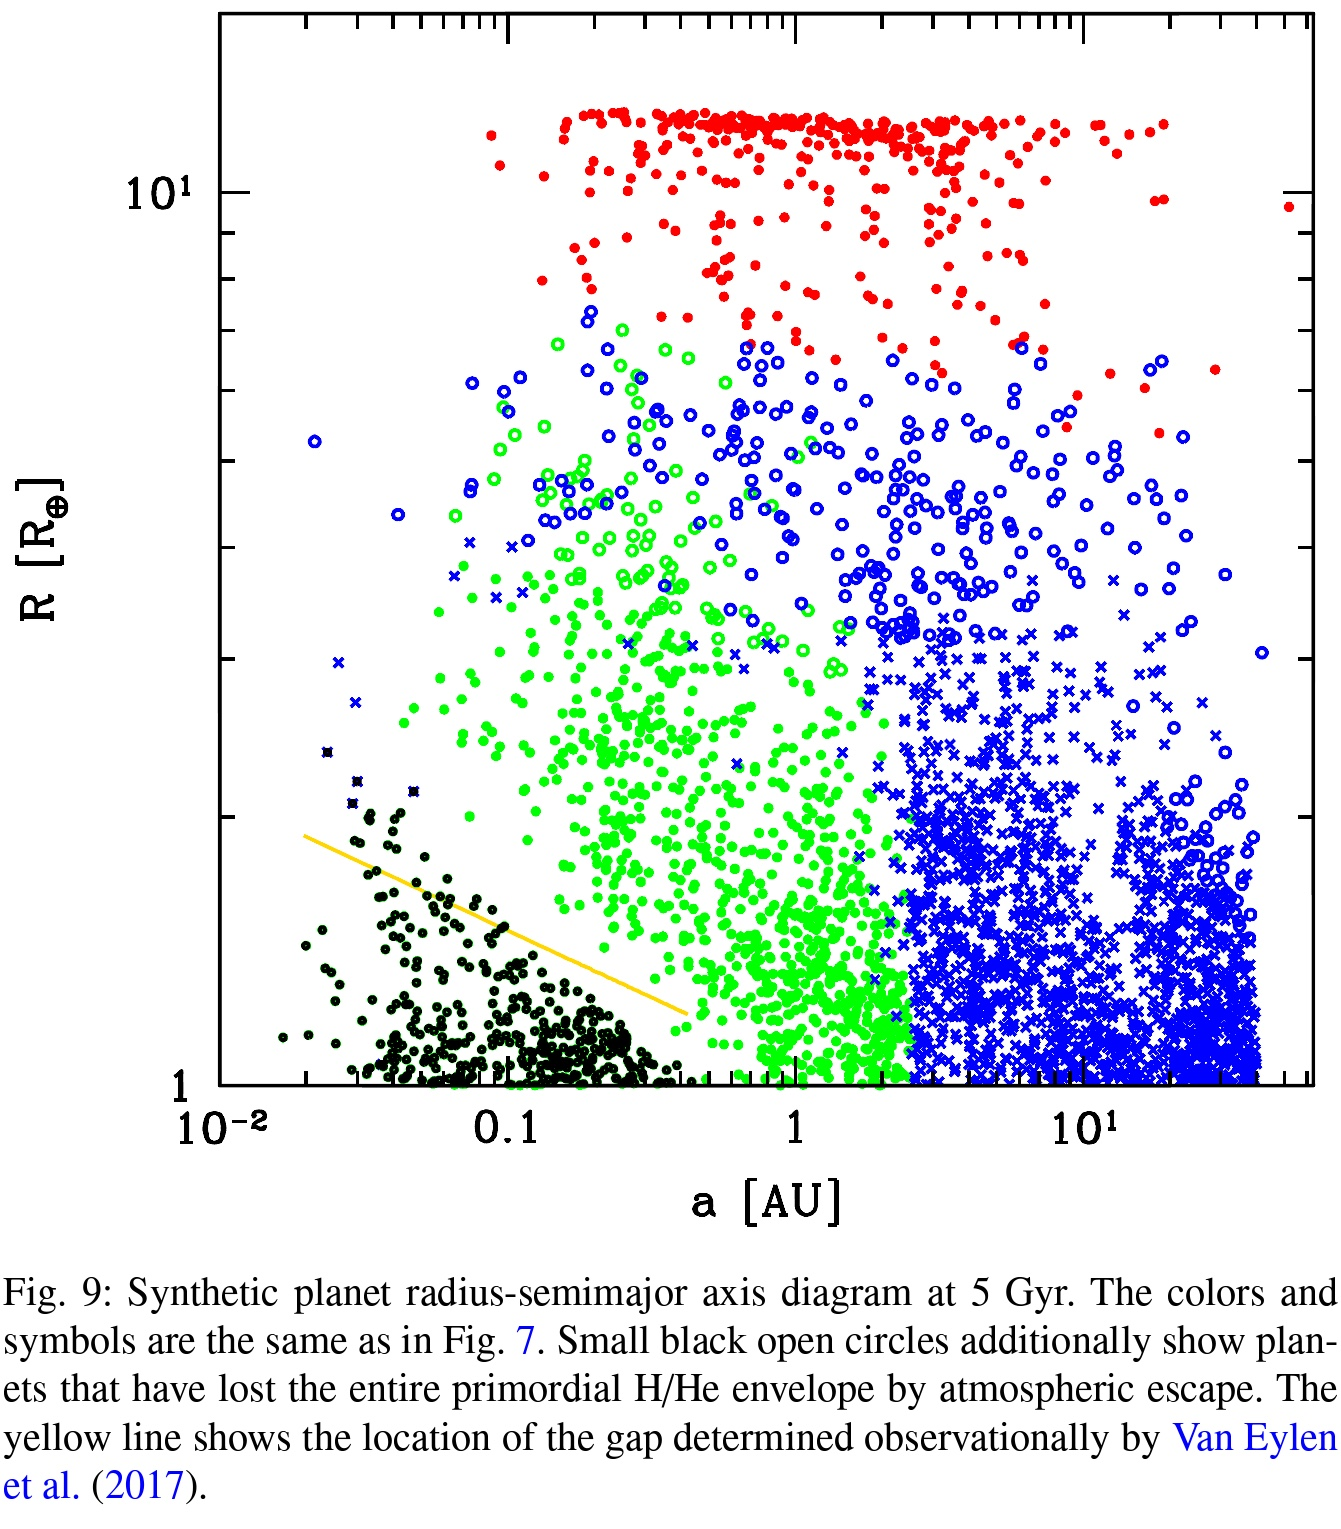
\includegraphics[trim={0.6cm 11cm 0.8cm 0.4cm},clip, keepaspectratio, width=0.99\textwidth]{Ra-synth}
	\caption{
		Da \cite{mordasini2018planetary}.}\label{fig:Ra-synth}
\end{figure}

Inoltre in figura (\ref{fig:ma-synth}) \'e evidente l'effetto della migrazione rapida all'interno: popolazione pianeti in origine nettuniani (frazione giaccio nel core $50\%$) che migrano all'interno accumulando materiale roccioso (frazione ghiaccio nel core $10-20\%$).

\begin{figure}[!ht]
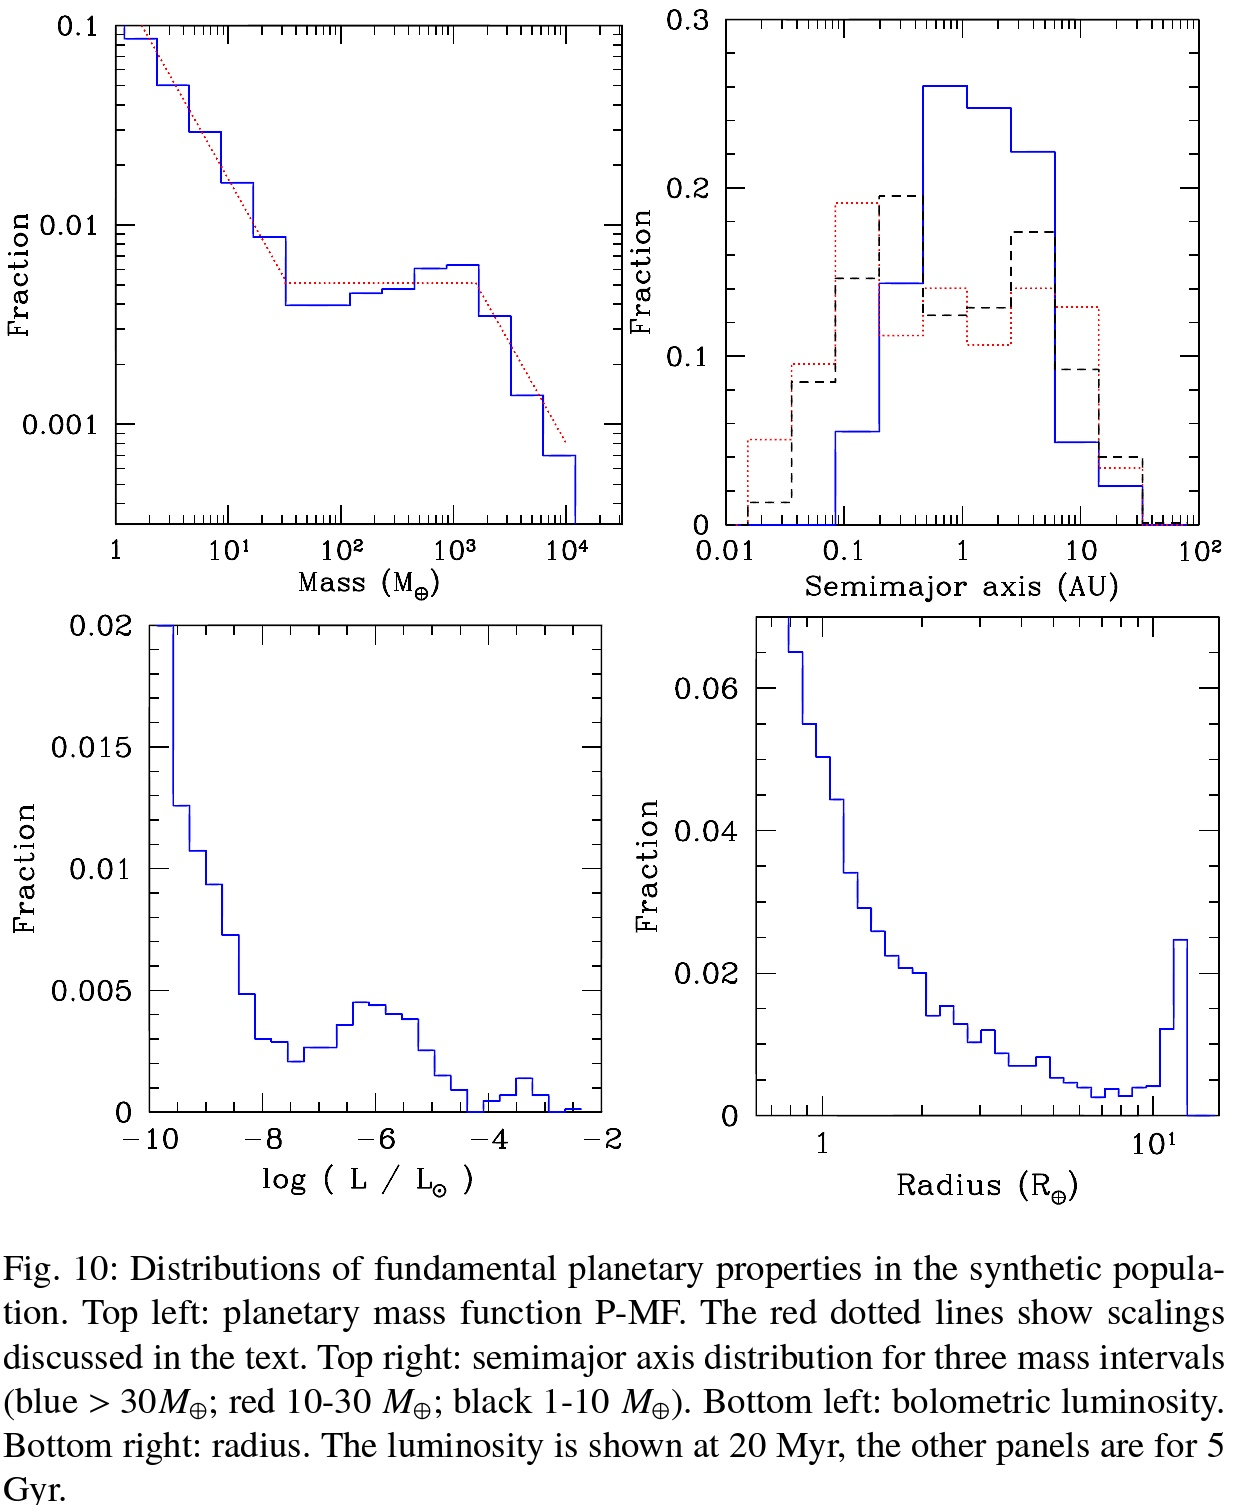
\includegraphics[trim={0cm 10cm 0 0},clip, width=0.9\textwidth,keepaspectratio]{MaLR-freq-synth}
\caption{Distribuzione di massa, semiasse, luminosit\'a, raggio. Da \cite{mordasini2018planetary}. }\label{fig:MaLR-freq-synth}
\end{figure}

\section{Caratteristiche delle distribuzioni delle propriet\'a fisiche dei pianeti e significativit\'a}

La figura (\ref{fig:MaLR-freq-synth}) mostra la distribuzione di massa di 509 pianeti della popolazione sintetica di \cite{mordasini2018planetary}. La distribuzione della massa dei pianeti ha andamento diverso per pianeti fino a $30\mearth{}$ formati principalmente da solidi e pianeti che hanno raggiunto la massa critica per l'accrescimento di gas runaway.
%La differente slope della distribuzione di massa nelle due regioni caratterizza i differenti meccanismi di accrescimento.
Si ha un minimo locale attorno alla massa critica dopo di che l'aumento di massa \'e molto veloce verso piccole masse. I risultati sono significativi per masse maggiori delle masse dell'embrione iniziale.

La distribuzione del raggio dei pianeti mostra picco a $1\rjupiter$ e crescita per piccoli raggi dovuta al loro lungo $\tkh{}$ e quindi scarso accrescimento di H/He.

La distribuzione dei semi-assi cresce rapidamente tra $0.01-0.1\si{\astronomicalunit}$, resta uniforme in log tra $0.1-10\si{\astronomicalunit}$ nonostante molti pianeti migrino all'interno,mentre i pianeti giganti sono ristretti in \SIrange{0.1}{6}{\astronomicalunit}. La distribuzioni del semiasse non mostra deviazioni dalla distribuzione iniziale.

%{\let\clearpage\relax\let\cleardoublepage\relax
%\chapter{Confronto semi-quantitativo tra caratteristiche popolazioni sintetiche e osservate}
%}

Per confrontare una popolazione planetaria simulata con le osservazioni \'e opportuno, oltre a tenere conto dei bias osservativi, valutare per quali sottoinsiemi dell'ensamble di pianeti ossevati le approssimazioni fatte nel modello sono valide.

%\section{Struttura orbitale e tipo di pianeta}

\begin{table}
\begin{tabular}{|ccc|}
\hline
N&Giganti ($M>300\mearth{}$)&vicini ($P\leq100\si{\day}, R\geq\rearth{}$)\\
\hline
1&4.8&8.4\\
2&7.4&12.8\\
3&5.4&11.4\\
4&0.4&10.0\\
$\geq5$&0.0&11.4\\
$\exv{S}$&18.0&54.0\\
O&10-20&50-60\\
\hline
\end{tabular}
\caption{Percentuale di stelle con N pianeti del dato tipo nella popolazione sintetica di \cite{mordasini2018planetary} e confronto con osservazioni.}\label{tab:planetfreq}
\end{table}

La posizione di Nettuno e Saturno nella figura (\ref{fig:ma-synth}) suggerisce che la posizione iniziale fosse probabilmente pi\'u interna (Grand-tack scenario).

La tabella (\ref{tab:planetfreq}) mostra un buon accordo tra teoria e osservazione per frequenza di pianeti giganti e sistemi compatti.

Il confronto della distribuzione di massa tra teorica e osservata mostra il buon accordo della pendenza nei due regimi di accrescimento e della posizione della massa critica. Per quanto riguarda la distribuzione dei raggi planetarii il picco a $1\rjupiter{}$ \'e meno pronunciato perch\'e sono inclusi solo pianeti giganti vicini e la distribuzione sintetica cresce meno rapidamente a piccoli raggi. Infine il gran numero di pianeti terrestri della popolazione sintetica pu\'o collidere dando luogo a pianeti pi\'u massicci tuttavia le interazioni dinamiche sono simulate solo per il tempo di vita del disco.

\begin{figure}[!ht]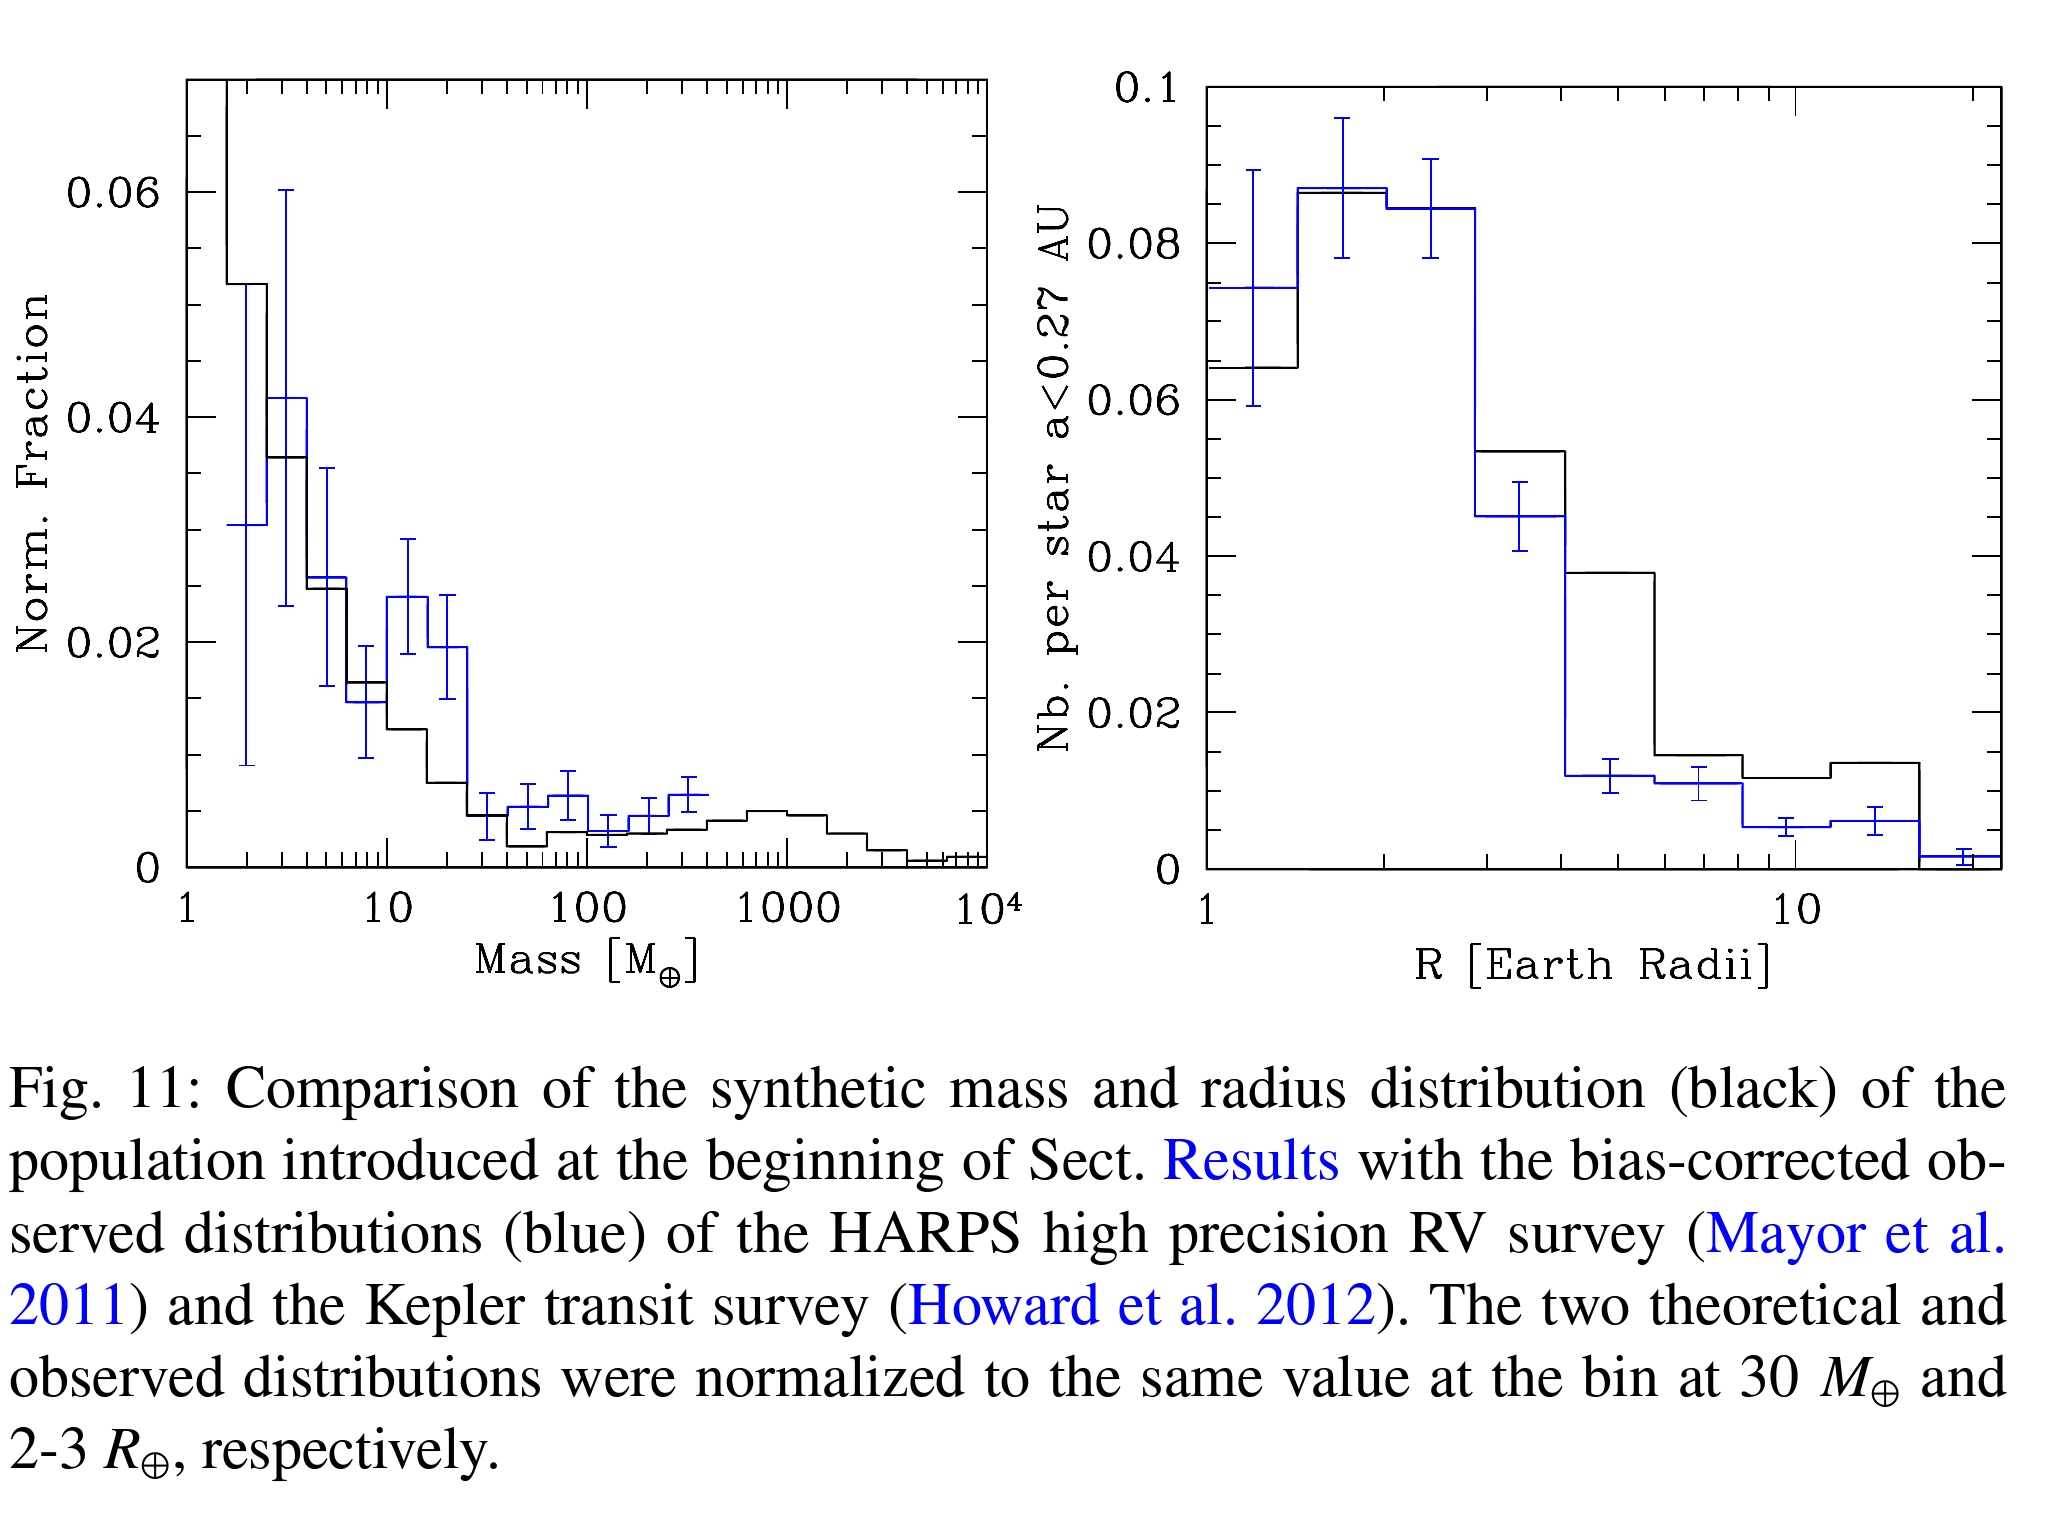
\includegraphics[trim={0cm 17cm 0 0},clip, keepaspectratio,width=0.9\textwidth]{MR-freq-obssynth}\caption{Distribuzioni di massa e raggio per popolazione planetaria sintetica (linea nera) e distribuzioni osservate tramite RV e transiti (linea blu) corrette per i bias. Da \cite{mordasini2018planetary}.}\label{fig:MR-freq-obssynth}\end{figure}

La probabilit\'a di osservare pianeti giganti aumenta con la metallicit\'a: la figura (\ref{fig:giant-Zsynth}) mostra che l'incremento relativo \'e in accordo con le osservazioni.

\begin{figure}[!ht]
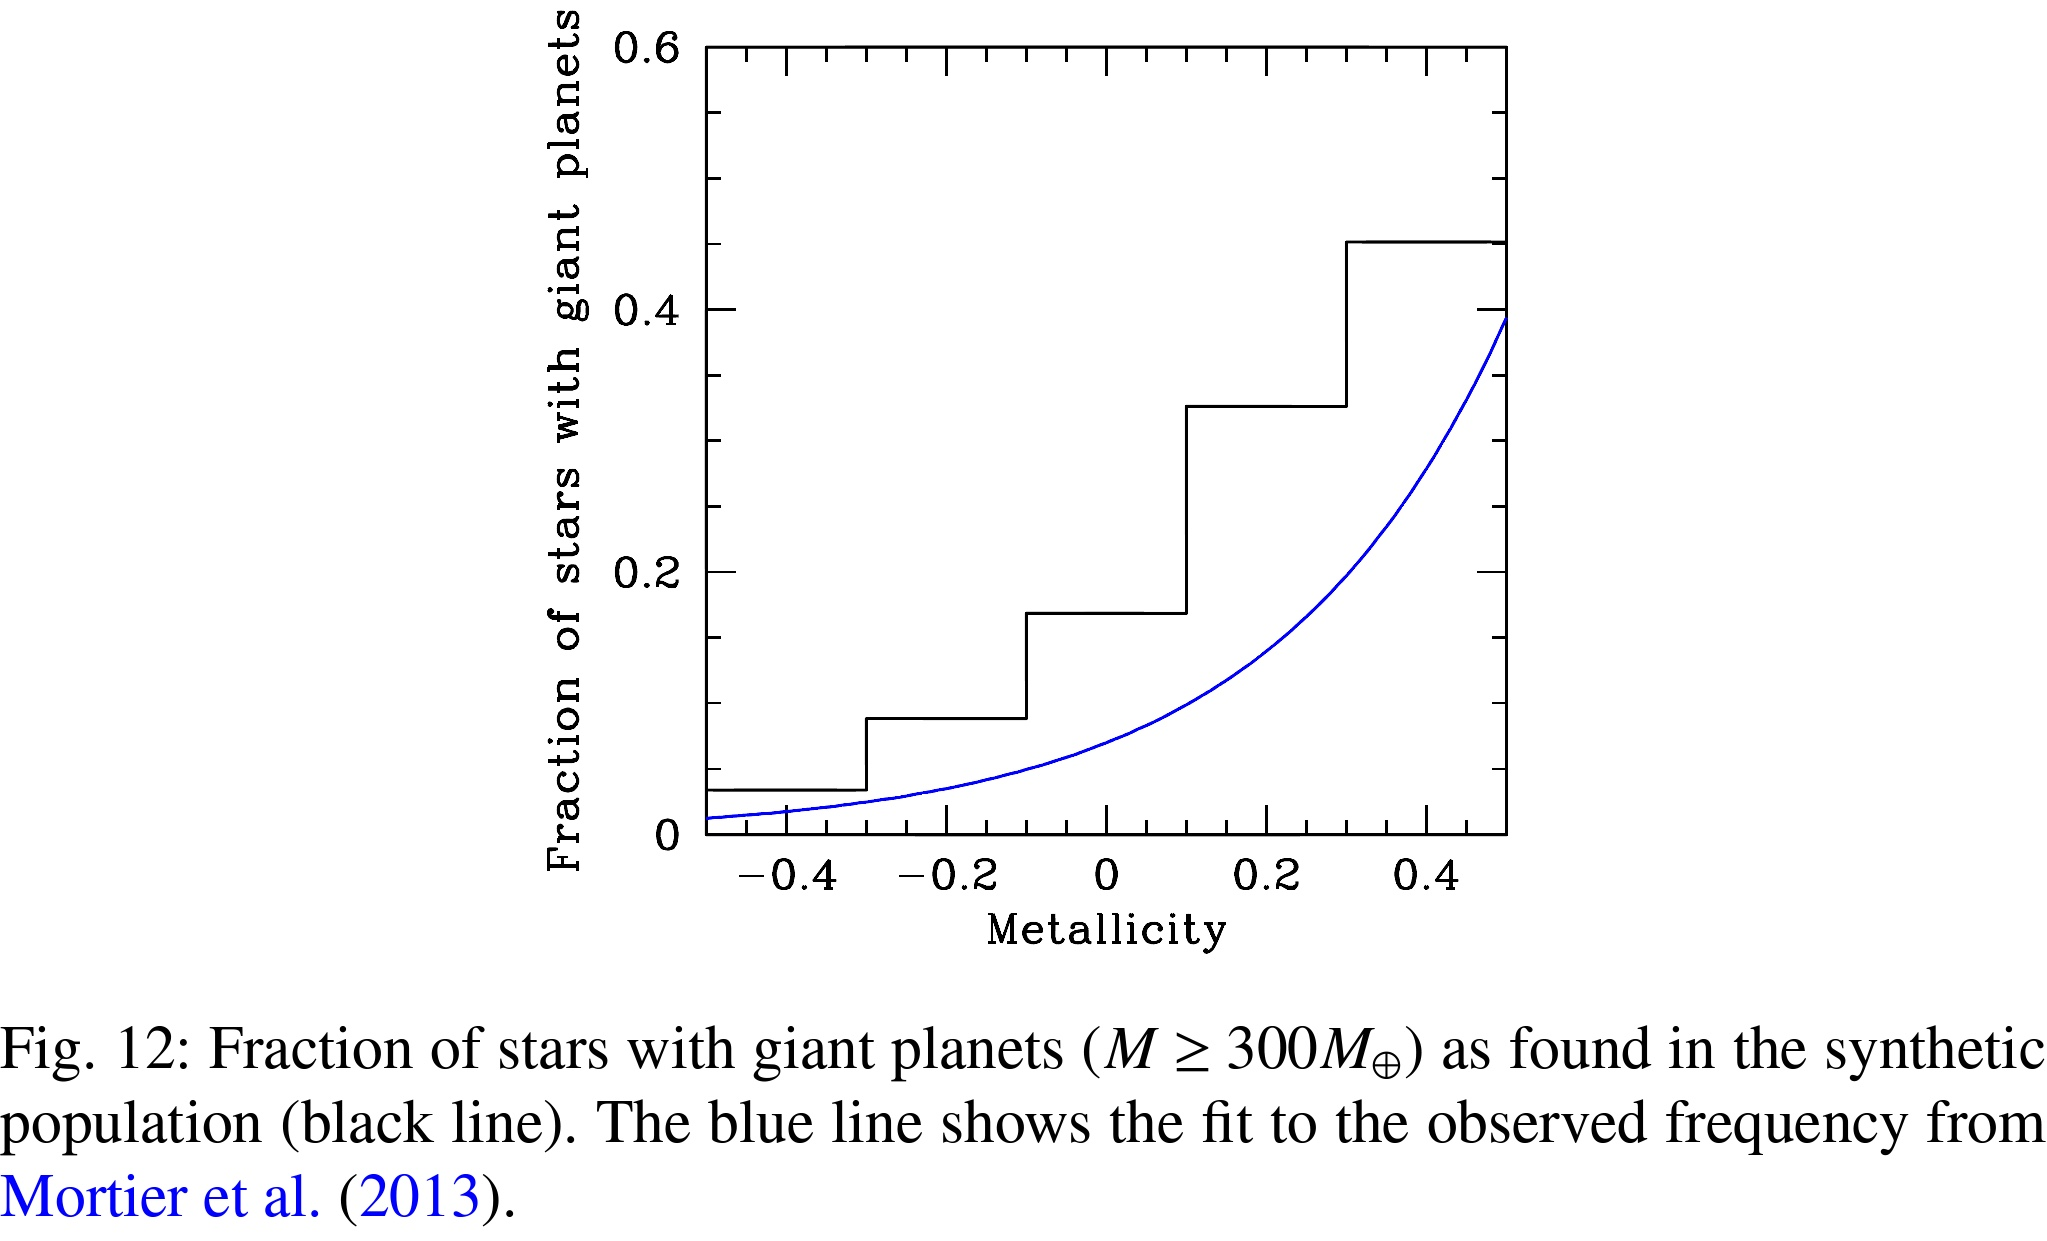
\includegraphics[trim={0cm 10cm 0 0},clip, width=0.9\textwidth,keepaspectratio]{giant-Zsynth}
\caption{Distribuzione di stelle che ospitano pianeti giganti ($M\geq300\mearth{}$) in funzione della metallicit\'a. Nero: popolazione sintetica. Blu: fit da osservazioni. Da \cite{mordasini2018planetary}. }\label{fig:giant-Zsynth}
\end{figure}

\begin{workout}[Distro luminosit\'a: relazione M-L]
	La distribuzione di luminosit\'a segue andamento $L\propto M^2$ con terzo picco per innesco deuterio a $\log{\frac{L}{\lsun}}\approx-3.5$
\end{workout}

\begin{workout}[Relazione $M_p$ vs $Z_p$]
	
\end{workout}

\begin{workout}[Relazione $Z_*$ metallicit\'a GP]
	
\end{workout}

\begin{workout}[Orbital structure and MMR: comparison simulation/observation]

\end{workout}

\begin{workout}[Comparison with stellar initial mass function]
Stelalr imf: chabrier 03, salpeter slope 1955
\end{workout}


%{\let\clearpage\relax\let\cleardoublepage\relax
%\chapter{Raffinamento dei modelli}
%}


\begin{workout}[Effects of saturation, cooling and irradiation.]
Impact of planet migration model on planetary populations: effects of saturation, cooling and stellar irradiation (??)
Outward migration helps some planets to become massive, accumulation zone at certain semiaxis, at what mass corotation saturate?
Migration of protoplanets in radiative disks
\end{workout}
